\documentclass[conference]{IEEEtran}
\IEEEoverridecommandlockouts
\usepackage{cite}
\usepackage{amsmath,amssymb,amsfonts}
\usepackage{graphicx}
\usepackage{textcomp}
\usepackage{xcolor}
\usepackage{tikz}
\usepackage{booktabs}
\usepackage{hyperref}
\usetikzlibrary{arrows.meta, positioning}

\def\BibTeX{{\rm B\kern-.05em{\sc i\kern-.025em b}\kern-.08em
    T\kern-.1667em\lower.7ex\hbox{E}\kern-.125emX}}

\begin{document}

\title{Medical Imaging AI Suite: A Multi-Modality Deep Learning System with Router-Based Dispatch and LLM-Assisted Interpretation}

\author{
\IEEEauthorblockN{Amit Mandal}
\IEEEauthorblockA{\textit{Senior Lecturer} \\
\textit{Dept. of Computer Science \& Engineering} \\
\textit{East West University} \\
amit.mandal@ewubd.edu}
\and
\IEEEauthorblockN{Khalilur Rahman Ridoy Khan}
\IEEEauthorblockA{\textit{Team Lead -- IT \& MIS Development} \\
\textit{GMGI Solutions Ltd.} \\
Dhaka, Bangladesh \\
khalilurrahmanridoykhan@gmail.com}
}

\maketitle

\begin{abstract}
This paper presents the Medical Imaging AI Suite, an educational multi-modality medical image classification system that unifies five independent deep-learning classifiers, covering chest X-ray pneumonia detection, CT lung-nodule malignancy classification, MRI brain-tumor classification, breast ultrasound lesion classification, and ECG arrhythmia classification, behind a single router. Each modality-specific model (ResNet18 transfer learning for the four imaging modalities, a dedicated architecture for the one-dimensional ECG waveform) was trained locally on an Apple M2 GPU (MPS) on public research datasets and evaluated with accuracy, AUROC, and confusion-matrix analysis. Test performance ranged from 81.0\% accuracy (CT, AUROC 0.854) to 95.1\% accuracy (MRI, AUROC 0.990), with X-Ray, Ultrasound, and ECG scoring 84.9\%/0.959, 91.0\%/0.987, and 86.9\%/0.977 respectively. A local large language model (via Ollama) is layered on top of each prediction to answer natural-language questions about the result without ever receiving the raw image, and a FastAPI/React web interface exposes the full predict-then-chat flow in a browser. The system is explicitly positioned as a learning and portfolio exercise: none of the five models is validated for clinical use.
\end{abstract}

\begin{IEEEkeywords}
medical imaging, deep learning, transfer learning, multi-modality classification, large language models, explainable AI
\end{IEEEkeywords}

\section{Introduction}
Medical imaging AI research typically treats each modality and each diagnostic task in isolation: one line of work on chest X-ray pneumonia detection, another on MRI tumor classification, another on ECG arrhythmia classification, each with its own pipeline and evaluation protocol. In practice, a single care pathway may touch several modalities for the same patient, and a practical decision-support tool would need to route an arbitrary input to the correct specialist model rather than assume one modality a priori.

This project investigates how far a single engineer, working with public datasets and commodity hardware, can go toward such a unified system. It builds five independent modality-specific classifiers (X-Ray, CT, MRI, Ultrasound, ECG), wraps them behind a shared router with one input/output contract, and adds a local large-language-model (LLM) layer that lets a non-technical user ask free-form questions about any one prediction, with the raw image or signal never leaving the machine.

The contributions of this work are:
\begin{enumerate}
\item Five trained deep-learning classifiers spanning four imaging modalities and one physiological-waveform modality, each with its own dataset, preprocessing pipeline, and documented test-set performance.
\item A modality-agnostic router abstraction that decouples model selection from model execution.
\item A local, no-API-key natural-language explanation layer over structured model predictions, built on an open-weight LLM (Ollama) rather than a cloud service, keeping data local.
\item A full predict-then-chat web application (FastAPI backend, React frontend) demonstrating the end-to-end flow.
\item An honest, quantitative account of each model's weaknesses (false-positive/false-negative trade-offs per modality), presented as a central finding rather than a caveat, consistent with the system's explicit non-clinical, educational framing.
\end{enumerate}

\section{Related Work}

\textbf{Chest X-ray pneumonia detection.} Rajpurkar et al.~\cite{chexnet} (CheXNet) trained a 121-layer CNN on the 112{,}120-image ChestX-ray14 dataset and reported performance exceeding the average of four practicing radiologists on pneumonia sensitivity and specificity. This established the pattern this project follows for X-Ray: a deep CNN fine-tuned on frontal chest radiographs, evaluated per-disease.

\textbf{CT lung-nodule malignancy classification.} Causey et al.~\cite{nodulex} (NoduleX) trained a CNN directly on CT nodule patches from LIDC-IDRI (over 1{,}000 nodules annotated by four thoracic radiologists) and reported an AUC near 0.99, comparable to expert radiologist agreement. The authors note that LIDC-IDRI's limited size constrains how sophisticated a model can be trained reliably, a limitation this project's own from-scratch 3D CNN on the smaller NoduleMNIST3D subset also runs into (Section~\ref{sec:discussion}).

\textbf{MRI brain-tumor classification.} Disci et al.~\cite{mri_cancers} fine-tuned six pretrained CNNs (Xception, MobileNetV2, InceptionV3, ResNet50, VGG16, DenseNet121) on the same four-class (glioma, meningioma, pituitary, no-tumor) public Brain Tumor MRI dataset used in this project, with Xception reaching 98.73\% weighted accuracy. The authors explicitly flag persistent difficulty raising recall on the glioma and meningioma classes, which matches this project's own finding that glioma is the weakest class (Section~\ref{sec:results}).

\textbf{Breast ultrasound lesion classification.} The BUSI dataset itself was introduced by Al-Dhabyani et al.~\cite{busi} (780 images, normal/benign/malignant, with lesion masks). A six-CNN benchmark on BUSI and UDIAT found EfficientNet strongest at 97.65\% accuracy and 96.30\% AUC; more recent work adds Grad-CAM-based explanations and targeted augmentation for the minority malignant class, the same class-imbalance issue this project's much smaller 780-image split also shows.

\textbf{ECG arrhythmia classification.} Kachuee et al.~\cite{kachuee} introduced the now-standard preprocessing this project reuses: segmenting the PhysioNet MIT-BIH Arrhythmia Database into fixed-length single-heartbeat windows and classifying them into the five AAMI EC57 classes (N, S, V, F, Q). Their residual CNN reported 93.4\% average accuracy on MIT-BIH; this project's own ECG model reaches 86.9\% overall accuracy with a similar per-class pattern, strongest on Q and F, weakest on S (Section~\ref{sec:results}).

\textbf{LLM-assisted explanation of imaging-model output.} A growing literature pairs a conventional CNN's prediction with a large language model that turns it into readable text, including saliency-grounded diagnostic narratives and anatomically-grounded multimodal explanation systems such as XMedGPT~\cite{xmedgpt}. A recurring open question in this literature is whether the LLM's text explanation is faithful to what the underlying model actually used, rather than a plausible-sounding but unverified narration. This project's chat layer (Section~\ref{sec:architecture}) takes a deliberately conservative approach to that risk: the LLM is never given the raw image for the prediction itself, only the classifier's structured output, so it can only narrate numbers already known to be correct.

\textbf{Gap this project addresses.} Each literature above optimizes one modality in isolation. This project's contribution is not a new state-of-the-art classifier in any single modality, but a unified, router-based system that dispatches across all five from one contract, paired with a local, privacy-preserving LLM explanation layer, an architecture uncommon in the single-modality literature reviewed above.

\section{System Architecture}
\label{sec:architecture}

The system has four layers, shown in Fig.~\ref{fig:architecture}.

\begin{enumerate}
\item A \textbf{router} (\texttt{router/registry.py}, \texttt{router/predict.py}) holds a single dictionary mapping a modality name to that modality's \texttt{predict(input\_path) -> \{label, confidence\}} function, so adding a sixth modality requires no change to any calling code.
\item Five \textbf{modality models}, each with its own \texttt{data.py}, \texttt{model.py}, \texttt{train.py} and \texttt{infer.py}: a ResNet18 fine-tuned per imaging modality (X-Ray, CT, MRI, Ultrasound) and a dedicated 1-D architecture for the ECG waveform. Each \texttt{infer.py} downloads its trained weights from a public Hugging Face Hub model repository on first use, so no binary weight file is committed to version control.
\item A \textbf{chat layer} (\texttt{chat/assistant.py}) runs the chosen model's prediction once, then opens a conversation with a local LLM served by Ollama (\texttt{qwen2.5-coder:7b} for text, \texttt{qwen2.5vl:7b} when an image is attached), seeded with a system prompt that states the prediction, the model's own documented accuracy and known weaknesses, and an explicit non-clinical disclaimer.
\item A \textbf{web UI}: a FastAPI backend exposes \texttt{/api/predict} and \texttt{/api/chat} over this same chat layer, with an in-memory session keyed by a UUID, and a React (Vite) frontend lets a user upload a file, pick a modality, see the prediction, and chat about it in a browser.
\end{enumerate}

All four layers run entirely on the local machine; no patient data or image leaves it.

\begin{figure}[t]
\centering
\resizebox{\columnwidth}{!}{%
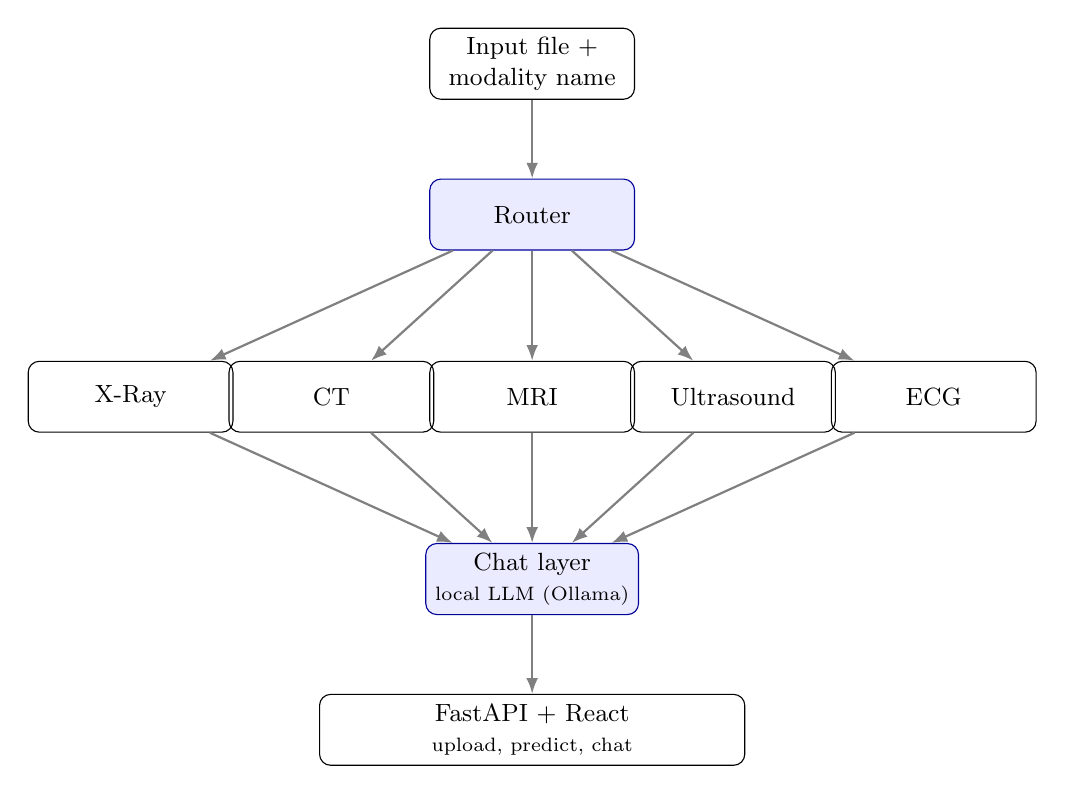
\begin{tikzpicture}[
  node distance=10mm and 6mm,
  box/.style={draw, rounded corners, minimum width=2.6cm, minimum height=0.9cm, align=center, font=\small},
  main/.style={box, draw=blue!60!black, fill=blue!8},
  arrow/.style={-{Latex[length=2mm]}, thick, gray}
]
\node[box] (input) {Input file +\\modality name};
\node[main, below=of input] (router) {Router};
\node[box, below=14mm of router, xshift=-5.1cm] (xray) {X-Ray};
\node[box, below=14mm of router, xshift=-2.55cm] (ct) {CT};
\node[box, below=14mm of router] (mri) {MRI};
\node[box, below=14mm of router, xshift=2.55cm] (us) {Ultrasound};
\node[box, below=14mm of router, xshift=5.1cm] (ecg) {ECG};
\node[main, below=14mm of mri] (chat) {Chat layer\\{\scriptsize local LLM (Ollama)}};
\node[box, below=10mm of chat, minimum width=5.4cm] (ui) {FastAPI + React\\{\scriptsize upload, predict, chat}};

\draw[arrow] (input) -- (router);
\draw[arrow] (router) -- (xray);
\draw[arrow] (router) -- (ct);
\draw[arrow] (router) -- (mri);
\draw[arrow] (router) -- (us);
\draw[arrow] (router) -- (ecg);
\draw[arrow] (xray) -- (chat);
\draw[arrow] (ct) -- (chat);
\draw[arrow] (mri) -- (chat);
\draw[arrow] (us) -- (chat);
\draw[arrow] (ecg) -- (chat);
\draw[arrow] (chat) -- (ui);
\end{tikzpicture}}
\caption{System architecture: the router dispatches an input to one of five modality models; each model's prediction is handed to a local-LLM chat layer, exposed to the user through a FastAPI/React web UI.}
\label{fig:architecture}
\end{figure}

\section{Methodology}

Table~\ref{tab:methods} summarizes the dataset, class set, backbone, and input format used for each modality.

\begin{table}[t]
\centering
\caption{Dataset and model summary per modality}
\label{tab:methods}
\footnotesize
\begin{tabular}{@{}p{1.3cm}p{2.0cm}p{1.6cm}p{1.9cm}@{}}
\toprule
\textbf{Modality} & \textbf{Dataset} & \textbf{Classes} & \textbf{Backbone} \\
\midrule
X-Ray & Kaggle chest X-ray pneumonia & Normal, Pneumonia & ResNet18 (pretrained) \\
CT & MedMNIST NoduleMNIST3D & Benign, Malignant & From-scratch 3D CNN \\
MRI & Kaggle Brain Tumor MRI & Glioma, Meningioma, Pituitary, No tumor & ResNet18 (pretrained) \\
Ultrasound & BUSI breast ultrasound & Normal, Benign, Malignant & ResNet18 (pretrained) \\
ECG & MIT-BIH (Kachuee preprocessing) & N, S, V, F, Q & 1-D CNN \\
\bottomrule
\end{tabular}
\end{table}

For the four imaging modalities, preprocessing follows the same pattern: resize to the model's trained resolution, convert to the channel count the backbone expects, convert to a tensor, and normalize with ImageNet mean/std ($[0.485, 0.456, 0.406]$ / $[0.229, 0.224, 0.225]$), exactly mirroring the transform used at training time so inference sees inputs from the same distribution the model was fit on. These parameters, together with the class list and input size, are saved once per modality as a metadata file and read back at prediction time, so preprocessing cannot silently drift from what training used.

Four backbones use \textbf{transfer learning}: a ResNet18 pretrained on ImageNet has its final fully-connected layer replaced with a new linear head and is then fine-tuned end-to-end on the modality's own training split, a standard, compute-efficient choice for small medical-imaging datasets consistent with the related-work backbones in Section~II. The CT and ECG models instead use smaller from-scratch architectures (a 3D CNN and a 1-D CNN respectively), reflecting their non-natural-image input shapes (a volumetric patch, a 1-D waveform) for which ImageNet pretraining does not transfer.

All five models were trained locally, selecting the best available device at runtime (CUDA, then Apple Silicon MPS, then CPU); every model in this project was trained on an Apple M2 (MPS backend), with the identical training script also runnable unmodified in Google Colab via a thin notebook wrapper. Trained weights are uploaded to a public Hugging Face Hub model repository rather than committed to version control, and are pulled down lazily on first inference.

\section{Experimental Setup}

Each modality uses its dataset's own standard train/validation/test split (the Kaggle-provided split for X-Ray and MRI, the official NoduleMNIST3D split for CT, a held-out split of BUSI for Ultrasound, and the inter-patient MIT-BIH split for ECG). Models were evaluated once on the held-out test split only, after training was complete; no test-set information was used for model selection or early stopping.

Three metrics are reported per modality: (1) \textbf{accuracy} on the test split; (2) \textbf{AUROC}, one-vs-rest and averaged for the multi-class modalities (MRI, Ultrasound, ECG), which is more informative than accuracy alone under class imbalance; and (3) \textbf{per-class confusion matrix}, from which per-class recall (sensitivity) is derived, since an aggregate accuracy figure can hide a model that performs well on a majority class and poorly on the minority class that matters clinically most (the malignant/pneumonia/arrhythmia classes).

All five test-set evaluations were computed by running each model's inference code against its held-out split, the same code path used at inference time, so the reported numbers reflect the deployed prediction pipeline rather than a separate offline evaluation script.

\section{Results}
\label{sec:results}

Table~\ref{tab:results} reports test accuracy and AUROC for all five modalities.

\begin{table}[t]
\centering
\caption{Test-set accuracy and AUROC per modality}
\label{tab:results}
\begin{tabular}{@{}lcc@{}}
\toprule
\textbf{Modality} & \textbf{Accuracy} & \textbf{AUROC} \\
\midrule
X-Ray & 84.9\% & 0.959 \\
CT & 81.0\% & 0.854 \\
MRI & \textbf{95.1\%} & \textbf{0.990} \\
Ultrasound & 91.0\% & 0.987 \\
ECG & 86.9\% & 0.977 \\
\bottomrule
\end{tabular}
\end{table}

MRI is the strongest model (95.1\% accuracy, 0.990 AUROC): the no-tumor and pituitary classes are classified correctly 99\%+ of the time, meningioma 98\%, but glioma only 82.5\% (330/400), most often confused with meningioma or no-tumor. CT is the weakest (81.0\% accuracy, 0.854 AUROC): it catches only 43 of 64 malignant test cases (67\% sensitivity), missing a third of malignant nodules, the most clinically costly error pattern in this project. X-Ray reaches high sensitivity for pneumonia (387/390, 99.2\%) but weak specificity on normal cases (143/234, 61.1\%), over-flagging healthy X-rays as pneumonia; the test split's distribution differs from the train/validation split for this specific Kaggle dataset, which explains why validation accuracy during training ($\sim$98\%) is far higher than the 84.9\% test figure reported here. Ultrasound catches 100\% of malignant test cases (21/21) but flags 3 of 14 normal cases as malignant, a false-alarm pattern that is the safer error direction on a very small (780-image) dataset. ECG shows the most balanced per-class recall across its five AAMI classes: N 85.9\%, S 78.2\%, V 87.8\%, F 92.0\%, Q 98.3\%, reasonable given the raw MIT-BIH data is roughly 83\% class N and under 1\% class F.

\section{Discussion}
\label{sec:discussion}

\textbf{Why MRI performs best.} The Brain Tumor MRI dataset has 7{,}023 images across four well-separated classes, the largest and most balanced of the five datasets used here, and the ResNet18 transfer-learning recipe matches what Disci et al.~\cite{mri_cancers} report as effective on the same dataset. The one weak class, glioma (82.5\% recall), mirrors their reported difficulty on exactly the same class, suggesting the confusion is a property of the data rather than a modeling mistake specific to this project.

\textbf{Why CT performs worst.} NoduleMNIST3D is small and imbalanced, and this project uses a from-scratch 3D CNN rather than transfer learning, since no ImageNet-style pretrained 3D backbone exists for this input shape. Causey et al.~\cite{nodulex} reach a much higher AUC ($\sim$0.99) on the same underlying LIDC-IDRI data, but with over 1{,}000 full-size nodules and access to radiomics features; this project's 81.0\% accuracy and 67\% malignant-class sensitivity on the smaller, pre-cropped subset is consistent with that gap, and is the single result in this suite that would need the most additional data and modeling work before being taken seriously even as a research baseline.

\textbf{Why X-Ray shows a train/test gap.} Validation accuracy during training reached roughly 98\%, but test accuracy is only 84.9\%. This is attributable to the specific Kaggle pneumonia dataset's test split coming from a different patient/imaging distribution than its train/validation split, a known quirk of this public dataset rather than overfitting introduced by this project's training recipe; the same fine-tuning recipe does not show a comparable gap on MRI or Ultrasound, which supports that explanation over a generic overfitting one.

\textbf{The common thread.} Every modality's weakest class is also its rarest or most visually ambiguous class in the training data: CT's malignant nodules, X-Ray's normal cases, ECG's class F (under 1\% of MIT-BIH), and MRI's glioma. This matches the wider literature reviewed in Section~II, where every paper that reports per-class numbers flags the same pattern, suggesting that for this class of problem, more and better-balanced data would move these numbers further than a different architecture would.

\textbf{On the LLM chat layer.} Because the chat layer seeds the LLM with the classifier's own documented accuracy and failure modes rather than letting it reason freely from the image, the explanation layer cannot produce the kind of unfaithful narration flagged as an open risk in the LLM-explanation literature (Section~II); the trade-off is that it can only discuss the specific prediction and its known statistics, not offer an independent visual read of the image.

\section{Limitations and Future Work}

\textbf{Not a clinical system.} Every model is trained on public research datasets for learning purposes. None is validated against an independent clinical population, none has regulatory clearance, and none should be used for real patient diagnosis or treatment decisions; this is stated explicitly in the project documentation and repeated in the LLM chat layer's system prompt so the disclaimer reaches the end user, not only the documentation.

\textbf{Scope limitations by design.} The CT model requires a pre-cropped $28\times28\times28$ nodule-candidate patch, not a whole CT volume; extracting candidate nodules from a full scan is a separate, substantially larger detection pipeline that is out of scope here. The ECG model requires a pre-segmented single 187-sample heartbeat, not a raw multi-beat strip; both choices isolate the classification problem this project targets from the upstream segmentation/detection problem, common practice in the benchmark literature (Section~II) but meaning neither model is a drop-in replacement for a full scan- or strip-level clinical tool.

\textbf{Remaining roadmap.} Two items remain open: automatic modality detection in the router, and a public demonstration interface. Both are deliberately deferred rather than abandoned and do not affect the validity of the trained models or their reported test-set numbers.

\textbf{Future work.} The most impactful next steps suggested by Section~\ref{sec:discussion}'s analysis would be: enlarging and rebalancing the CT training set (or adding radiomics features as in~\cite{nodulex}); investigating the X-Ray dataset's train/test distribution shift directly rather than only documenting it; and, in line with the open question raised in the LLM-explanation literature (Section~II), a systematic check of whether the chat layer's natural-language answers stay faithful to the underlying classifier's actual confidence and failure modes under adversarial questioning.

\section{Conclusion}

This paper described the Medical Imaging AI Suite, a five-modality medical image classification system (X-Ray, CT, MRI, Ultrasound, ECG) unified behind a single router, with a local LLM layer that explains each prediction in natural language and a FastAPI/React web application exposing the full flow. Test-set performance ranged from 81.0\% accuracy / 0.854 AUROC (CT) to 95.1\% accuracy / 0.990 AUROC (MRI), and the per-class analysis in Sections~\ref{sec:results}--\ref{sec:discussion} showed that every modality's weakest class is also its rarest or most visually ambiguous one in the training data, a pattern consistent with the published literature on each individual task. The project's main contribution is architectural rather than a new state-of-the-art classifier: a shared, modality-agnostic router contract and a privacy-preserving, locally-run explanation layer that together demonstrate, on commodity Apple-Silicon hardware and entirely public datasets, how far a single-engineer educational project can go toward the kind of unified, multi-modality decision-support tool that the existing single-modality literature does not by itself provide. As stated throughout, the resulting system remains a learning and portfolio exercise, not a clinical tool.

\begin{thebibliography}{00}

\bibitem{chexnet} P. Rajpurkar et al., ``CheXNet: Radiologist-Level Pneumonia Detection on Chest X-Rays with Deep Learning,'' \textit{arXiv preprint arXiv:1711.05225}, 2017.

\bibitem{nodulex} J. L. Causey et al., ``Highly accurate model for prediction of lung nodule malignancy with CT scans,'' \textit{Scientific Reports}, vol. 8, p. 9286, 2018.

\bibitem{mri_cancers} R. Disci, F. Gurcan, and A. Soylu, ``Advanced Brain Tumor Classification in MR Images Using Transfer Learning and Pre-Trained Deep CNN Models,'' \textit{Cancers}, vol. 17, no. 1, p. 121, 2025.

\bibitem{busi} W. Al-Dhabyani, M. Gomaa, H. Khaled, and A. Fahmy, ``Dataset of breast ultrasound images,'' \textit{Data in Brief}, vol. 28, p. 104863, 2020.

\bibitem{kachuee} M. Kachuee, S. Fazeli, and M. Sarrafzadeh, ``ECG Heartbeat Classification: A Deep Transferable Representation,'' \textit{arXiv preprint arXiv:1805.00794}, 2018.

\bibitem{xmedgpt} ``XMedGPT: a grounded multimodal medical assistant,'' \textit{arXiv preprint arXiv:2505.06898}, 2025.

\end{thebibliography}

\end{document}
